\subsection*{\textbf{> О чём это руководство?}}
\addcontentsline{toc}{subsection}{О чём это руководство?}
\vspace{-0.5cm}

Это небольшой путеводитель в мир Debian. На самом деле это просто собрание моих
заметок и ссылок, накопившихся за годы работы с Debian. В этом руководстве я
рассказываю о том, как начать вносить вклад в Debian, разобраться в первых шагах
в проекте и со временем прийти к роли DM (Debian Maintainer). Когда-то мне
самому очень не хватало такого руководства под рукой, чтобы двигаться вперёд не
методом тыка, а более последовательно и осознанно.

\vspace{-0.5cm}
\subsection*{\textbf{> Для кого это руководство?}}
\addcontentsline{toc}{subsection}{Для кого это руководство?}
\vspace{-0.5cm}

Это руководство для тех, кто хочет начать участвовать в Debian, но пока не
знает, с чего начать, как устроен проект и какие практические шаги можно
предпринять на старте.

Руководство рассчитано на читателя, который уже знаком с базовыми инструментами
разработки и работы в GNU/Linux. Предполагается, что вы умеете пользоваться Git,
платформами GitLab/GitHub, командной строкой и текстовым редактором, понимаете
основы сборки программ и Debian-пакетов и в целом достаточно уверенно работаете
с Debian как пользователь. Также предполагается, что вы владеете языком
программирования или скриптовым языком, который хотите использовать для участия
в Debian, имеете электронную почту для общения, умеете пользоваться
ИИ-инструментами при необходимости и хотя бы немного знаете английский язык.

\vspace{10cm}

Если каких-то знаний пока не хватает, можно сначала разобраться в следующих
темах. Не стоит с головой уходить в документацию --- на старте достаточно знать
основы/базовые вещи.

\textbf{Начальный уровень}

\textcolor{teal}{> The Debian Trixie beginner's handbook}

PDF (EN): \url{https://debian-beginners-handbook.arpinux.org/trixie-en/download/the_beginners_handbook.pdf}

Web (EN): \url{https://debian-beginners-handbook.arpinux.org/trixie-en/the_beginners_handbook.html}

\textcolor{teal}{> Руководство по установке Debian GNU/Linux}

Web (RU): \url{https://www.debian.org/releases/trixie/amd64/index.ru.html}

Web (EN): \url{https://www.debian.org/releases/trixie/amd64/index.en.html}

\textcolor{teal}{> Настольная книга администратора Debian}

Web (RU): \url{https://www.debian.org/doc/manuals/debian-handbook/index.ru.html}

Web (EN): \url{https://www.debian.org/doc/manuals/debian-handbook/index.en.html}

\textbf{Средний уровень}

\textcolor{teal}{> Руководство начинающего разработчика Debian}

Web (RU): \url{https://www.debian.org/doc/manuals/maint-guide/index.ru.html}

Web (EN): \url{https://www.debian.org/doc/manuals/maint-guide/index.en.html}

\textcolor{teal}{> Руководство для сопровождающих Debian}

Web (RU): \url{https://www.debian.org/doc/manuals/debmake-doc/index.ru.html}

Web (EN): \url{https://www.debian.org/doc/manuals/debmake-doc/index.en.html}

\textcolor{teal}{> Руководство по созданию пакетов Debian}

PDF (RU): \url{https://www.debian.org/doc/manuals/packaging-tutorial/packaging-tutorial.ru.pdf}

PDF (EN): \url{https://www.debian.org/doc/manuals/packaging-tutorial/packaging-tutorial.en.pdf}

\vspace{10cm}

\textcolor{teal}{> APT User's Guide}

Web (EN): \url{https://www.debian.org/doc/manuals/apt-guide/index.en.html}

\textcolor{teal}{> Securing Debian Manual}

Web (EN): \url{https://www.debian.org/doc/manuals/securing-debian-manual/index.en.html}

\textcolor{teal}{> Часто задаваемые вопросы о Debian GNU/Linux}

Web (RU): \url{https://www.debian.org/doc/manuals/debian-faq/index.ru.html}

Web (EN): \url{https://www.debian.org/doc/manuals/debian-faq/index.en.html}

\textbf{Продвинутый уровень}

\textcolor{teal}{> Debian Reference}

Web: \url{https://www.debian.org/doc/manuals/debian-reference/}

\textcolor{teal}{> Debian Policy Manual}

Web: \url{https://www.debian.org/doc/debian-policy/}

\textcolor{teal}{> Debian Developer's Reference}

Web: \url{https://www.debian.org/doc/manuals/developers-reference/}

\textcolor{teal}{> Debian Hamradio Maintainer's Guide}

Web: \url{https://www.debian.org/doc/manuals/hamradio-maintguide/}

\vspace{-0.5cm}
\subsection*{\textbf{> Зачем вносить вклад в Debian и в FOSS в целом?}}
\addcontentsline{toc}{subsection}{Зачем вносить вклад в Debian и в FOSS в целом?}
\vspace{-0.5cm}

Вносить вклад в Debian и в FOSS --- это не только про то, чтобы "починить пакет
для себя". Это возможность сделать лучше инструмент, которым будут пользоваться
тысячи людей. Особенно приятно потом самому использовать систему и знать, что в
ней есть и твоя работа: исправление, перевод, идея или улучшение.  Такой вклад
дает чувство участия в чем-то большом, где твои усилия действительно приносят
пользу.

При этом вклад в Debian часто выходит далеко за пределы самого Debian:
исправления и улучшения со временем попадают и в другие дистрибутивы, такие как
Ubuntu, Linux Mint, Kali Linux, Pop!\_OS, MX Linux, PureOS и многие другие.
Значит, помогая Debian, вы помогаете всей экосистеме свободного ПО. И в этом
есть нечто большее: это вклад в будущее, в открытую культуру знаний и
технологий, частью которой вы становитесь сами.

\vspace{10cm}

\begin{center}
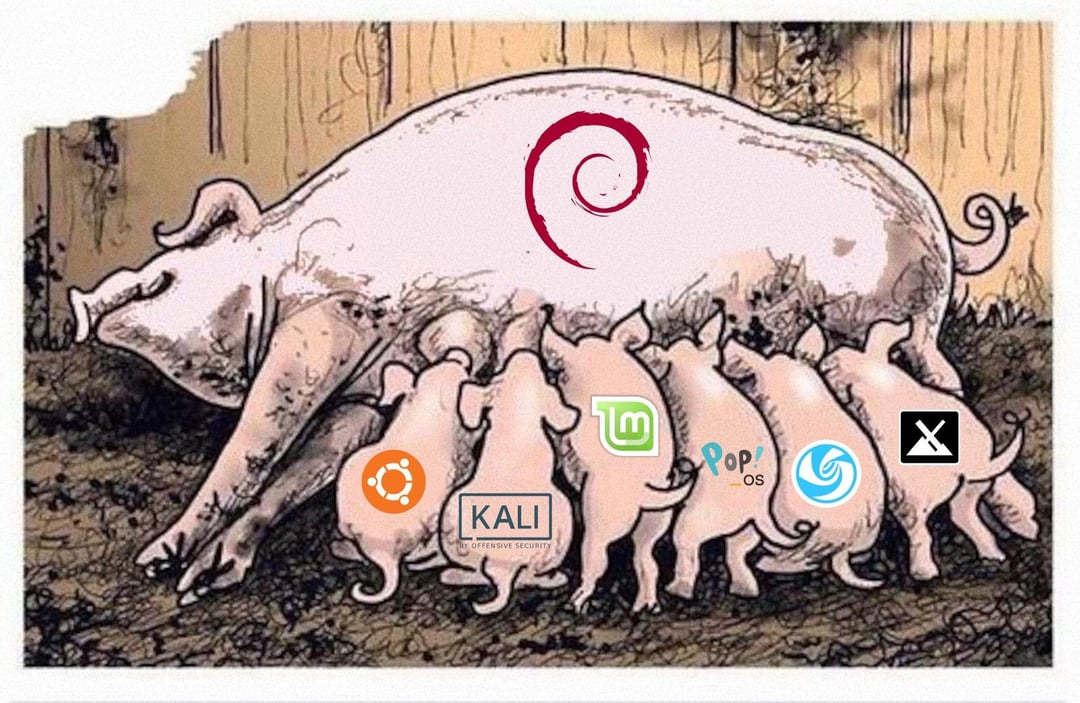
\includegraphics[width=0.70\textwidth]{images/forks.jpg}

\small \textbf{Потомки Debian}

\vspace{1cm}

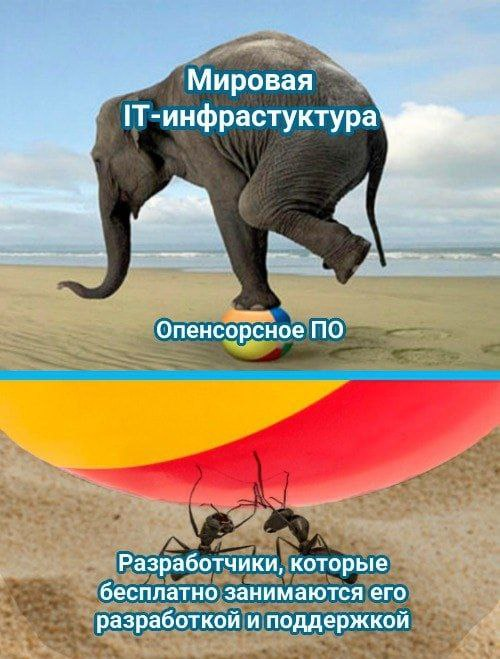
\includegraphics[width=0.70\textwidth]{images/motivation.jpg}

\small \textbf{Мотивация}
\end{center}
